\chapter{Centro de Inteligência}\label{cap_trabalho_academico}

Antes de avançar para a parte técnica, é importante explicar o que é o Centro de Inteligência da JFRN e como um painel poderia ajudar na tarefa deles.

De acordo com o site do Centro de Inteligência, ele existe para otimizar o trabalho jurisdicional a partir de demandas repetitivas. Esse tipo de demanda deve ser comunicado às autoridades para que a multiplicação desses casos diminuam, e não haja uma sobrecarga. 

A partir disso começou a pesquisa para decidir qual seria a ferramenta escolhida para desenvolver o painel, e como o painel precisava ter um desenvolvimento rápido e simples, para ser facilmente distribuído, foi decidido usar a linguagem de programação Python.

\section{Python}

Python é uma linguagem de programação de alto nível e de aplicações gerais, foi criada por Guido van Rossum e lançada em 1991. Suporta vários paradigmas, incluindo orientação a objeto e programação funcional. Essas características a tornaram muito popular entre programadores, porque é possível construir muita coisa usando poucas linhas de código, e esses projetos vão desde um timer simples, até grandes análises de dados e sistemas com inteligência artificial.

No final do capítulo 1 foram detalhadas algumas ferramentas BI, entre elas Tableau e Power BI, essas ferramentas já vem prontas com todas as funcionalidades que o usuário vai precisar, já lê os dados automaticamente, identifica campos e cria gráficos de forma muito rápida, porém os custos de implementação são altos, as licenças também são caras e é difícil encontrar profissionais que mexam nessas ferramentas tão específicas. Já no Python alguns desses problemas são resolvidos, o Python é uma linguagem de programação, portanto não tem nada pronto, tudo precisa ser construído, desde o leitor de dados, até o construtor de gráficos, o trabalho para se desenvolver um painel usando uma linguagem de programação é difícil, mas uma vez desenvolvido, é muito fácil de se manter, e o custo é zero porque não há licenças que limitem a quantidade de usuários que podem acessar o que foi feito. Além disso, é relativamente fácil encontrar desenvolvedores de Python no Rio Grande do Norte (e no Brasil), porque é uma linguagem muito usada no mundo todo, isso pode ser visto no ranking elaborado pelo \textit{Institute of Electrical and Electronics Engineers} (IEEE).

Portanto, o uso do Python para elaborar um painel pode ser difícil no início, porque muita coisa precisa ser construída do zero, mas uma vez que isso esteja desenvolvido é, relativamente, fácil de se manter porque não há custos envolvidos com o uso da ferramenta em si. Apesar disso, um dos problemas seria o suporte, nas opções pagas é possível requisitar suporte caso alguma coisa não funcione, já no Python se acontecer algum imprevisto, os próprios desenvolvedores é que devem solucionar.

\begin{figure}[h]
	\centering
	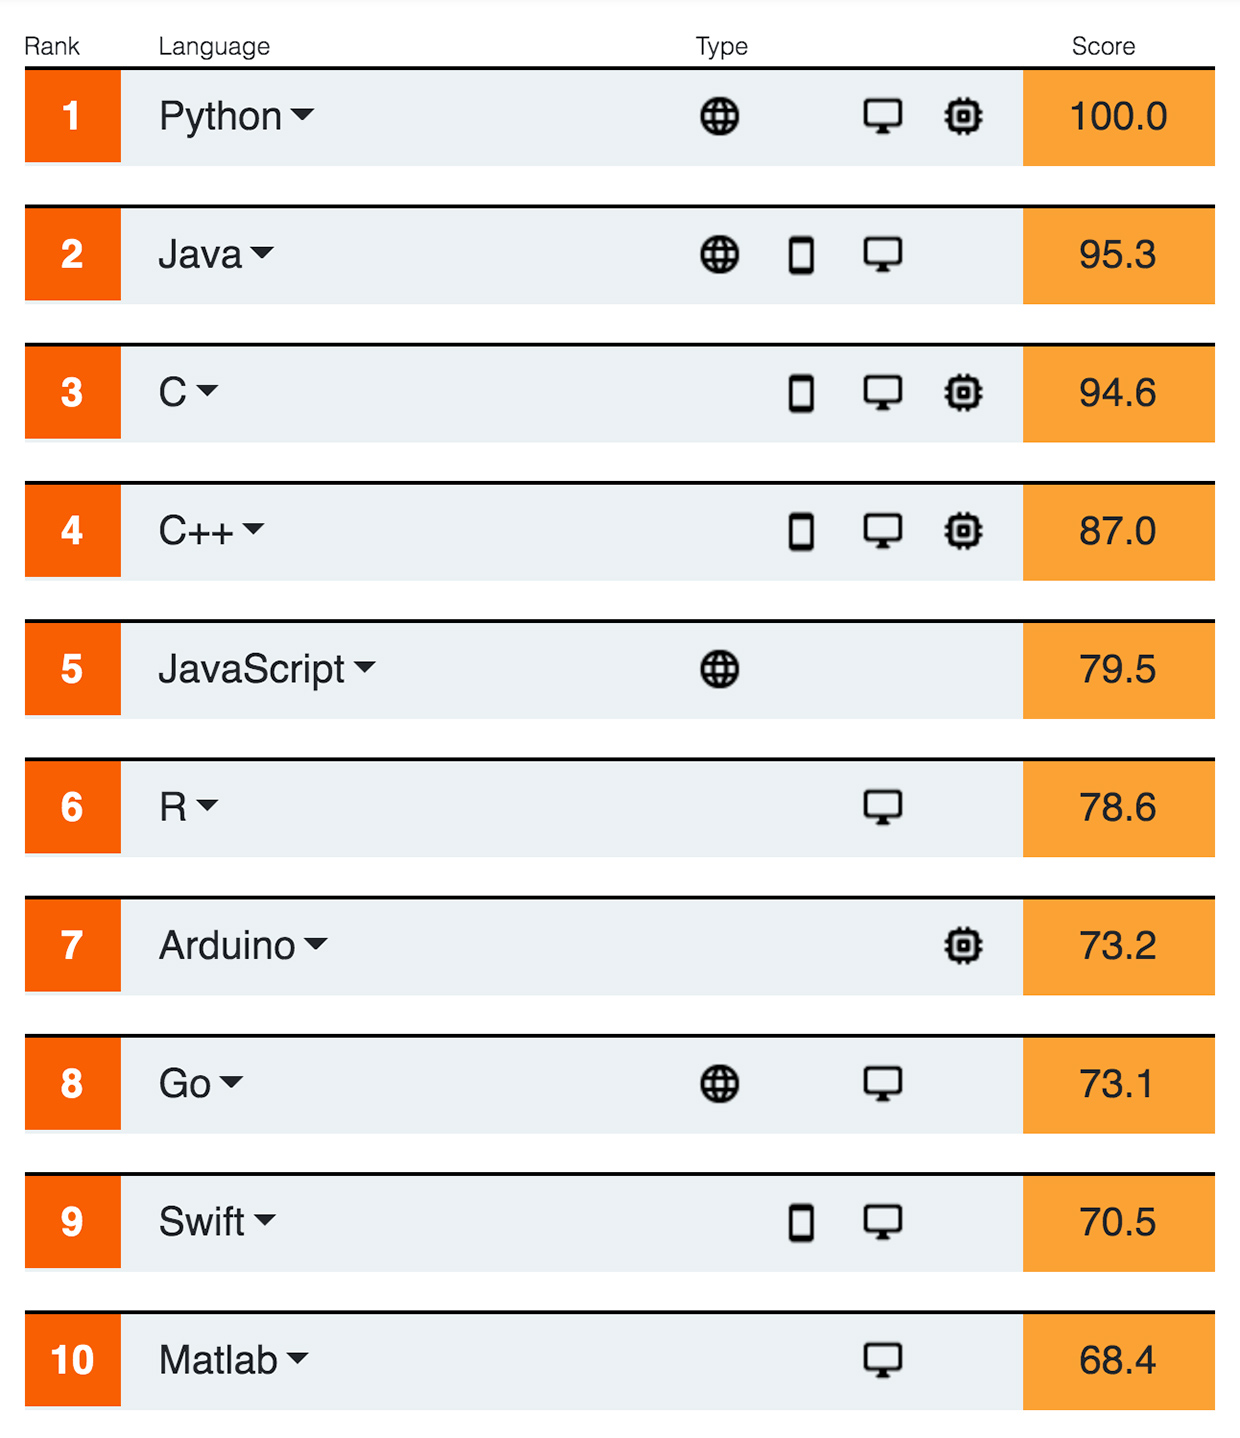
\includegraphics[scale=0.25]{./figures/cap2/ranking_python.jpeg}
	\caption{Linguagens de programação mais usadas em 2020}
\end{figure}

Outro ponto positivo de se usar Python é a replicabilidade, é possível criar painéis que atendam as diferentes Varas da JFRN, mostrando os dados que os gestores preferirem e acharem que são mais relevantes para suas realidades.

\section{Estrutura básica do painel}

Com os dados da JFRN em mãos e a ferramenta escolhida, passou-se a pesquisar quais seriam as bibliotecas usadas, portanto, a estrutura ficou da seguinte forma:

\begin{figure}[h]
	\centering
	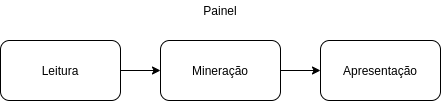
\includegraphics[scale=0.65]{./figures/cap2/estrutura_painel.png}
	\caption{Estrutura básica do painel}
\end{figure}

O painel que se propôs ao Centro de Inteligência não tem a estrutura clássica com diferentes tabelas (fato e dimensão), com as quais se geram as visualizações, no lugar disso, existe um arquivo .csv que contém os dados que serão usados, esses dados .csv fazem parte uma extração que veio do PJe, e a partir desse arquivo o painel vai criar subconjuntos de acordo com o ano e órgão julgador escolhidos pelo usuário.